%% IEEE Conference Paper
%% Orbital Sentinel: Foster B-Plane Conjunction Assessment Prototype
%% Compile: pdflatex -> pdflatex  (bibtex not required; thebibliography used)
%%
%% FIX LOG
%%  - Removed all Unicode box-drawing characters (en/em dashes in comments)
%%    that caused "Missing number" on line 42 and similar errors.
%%  - Replaced V\&V with V\&{}V to avoid ligature issues.
%%  - Tightened tabular column widths to eliminate overfull hboxes.
%%  - Added three figures using pgfplots (no external images required).
%%  - Resynced with the September 2026 audit: eleven defects (was four/five),
%%    116 tests (was three), corrected risk-scorer metrics 75.46%/44.64% recall
%%    (was 93.85% from a model outside the request path), and distinct GAT
%%    metrics 95.54% (was a byte-identical copy of the GNN row).
%%  - Corrected the maneuver burn unit from km/s to m/s and separated the two
%%    distinct burn computations (planner vs ranker-internal).
%%  - Corrected cascade depth to include the influence term.
%%  - Renamed the regression table label to avoid a stale \ref.

\documentclass[conference]{IEEEtran}

\usepackage{amsmath}
\usepackage{amssymb}
\usepackage{graphicx}
\usepackage{url}
\usepackage{booktabs}
\usepackage{multirow}
\usepackage{cite}
\usepackage{xcolor}
\usepackage{tikz}
\usepackage{pgfplots}
\pgfplotsset{compat=1.18}
\usepackage{pgfplotstable}
\usepackage{hyperref}
\hypersetup{colorlinks=true, linkcolor=blue, citecolor=blue, urlcolor=blue}

%% Convenience macros
\newcommand{\norm}[1]{\left\|#1\right\|}
\newcommand{\bvec}[1]{\mathbf{#1}}
\newcommand{\Pc}{P_c}
\newcommand{\RHBR}{R_{\mathrm{HBR}}}
\DeclareMathOperator{\tr}{tr}

%% Suppress pgfplots warnings in IEEE two-column mode
\pgfplotsset{
  every axis/.append style={font=\footnotesize},
  scaled ticks=false
}

%% ============================================================
\begin{document}

\title{Orbital Sentinel: Explainable Real-Time Conjunction Assessment\\
with Foster B-Plane Integration, Hermite TCA Refinement,\\
and Layered Debris Forecasting}

\author{%
  \IEEEauthorblockN{[Author Names]}\\
  \IEEEauthorblockA{[Institution / Department]\\
  [City, Country]\\
  [email addresses]}
}

\maketitle

%% Abstract
\begin{abstract}
Orbital Sentinel is a prototype for real-time satellite tracking, conjunction
awareness, risk ranking, and three-dimensional incident visualization. The system
integrates Two-Line Element~(TLE) ingestion, SGP4 propagation, a FastAPI service
layer, and a Cesium-based WebGL client. The collision-probability path implements
the Foster~(1992) B-plane double-integration method with a
Radial/Transverse/Normal~(RTN) covariance model and a Chan~(1997) series fallback;
risk ranking uses an XGBoost classifier trained on Foster-generated synthetic data
alongside two graph cascade rankers---a deterministic surrogate over graph summary
statistics and a multi-head graph attention network---for maneuver probability and
cascade depth. This paper documents the full implemented methodology, identifies
and corrects eleven material defects, and evaluates the corrected paths through a
116-test regression suite. Five defects concern the physics and rendering path:
miss-independent probability, sample-grid TCA error, initial-epoch hotspot
placement, debris generated for near-misses, and loss of multi-layer debris
rendering. Six concern the learned and disseminated results: an attention ranker
that reported another model's scores as its own, an alert pipeline disabled under
the default configuration, ranker failure converted into a plausible all-zero
plan, risk-scorer metrics drawn from a model outside the request path, alert
count and list able to disagree, and TCA urgency measured against wall-clock
time. Cached evaluation on Foster-derived synthetic data yields 75.46\% accuracy
at 44.64\% recall for the production risk scorer, 98.76\% for the surrogate ranker,
and 95.54\% for the attention ranker. These figures characterize internal
synthetic-set behavior and are not operational flight-validation claims.
\end{abstract}

\begin{IEEEkeywords}
space situational awareness, conjunction assessment, SGP4, Foster collision
probability, B-plane integration, time of closest approach, debris visualization,
cascade risk, graph neural networks, XGBoost
\end{IEEEkeywords}

%% =============================================================
\section{Introduction}
\label{sec:intro}

The cataloged orbital population now exceeds 27\,000 tracked objects, and the
estimated population of lethal untracked debris fragments numbers in the hundreds
of thousands~\cite{esa2024}. As constellation deployment accelerates, the number
of object pairs requiring daily screening grows quadratically with catalog size,
placing increasing pressure on Space Situational Awareness~(SSA) infrastructure.
Prototype systems that expose the geometry, timing, uncertainty, and downstream
consequences of encounters in a transparent, debuggable architecture serve an
important role: they allow methodology auditing, operator training, and controlled
comparison of algorithmic choices before operational commitment.

Orbital Sentinel addresses this need with an end-to-end pipeline: orbital states
are propagated from TLEs via SGP4, cached, screened for close approaches, ranked
by risk, streamed over WebSocket at 1~Hz, and rendered on an interactive Cesium
globe. The system contains demo-specific logic, synthetic machine-learning
artifacts, and a test router for injecting deterministic encounter scenarios.
These components impose a precise reporting obligation---implementation outputs
must not be conflated with operationally validated collision probabilities. This
paper enforces that boundary throughout.

\subsection*{Research Questions}
\begin{enumerate}
  \item Does collision probability respond to both positional uncertainty and the
        relative miss vector in the B-plane?
  \item Can the TCA routine detect a close approach occurring between coarse
        numerical output samples?
  \item Are hotspot and debris products located at the computed TCA position
        rather than the initial epoch?
  \item Does the Cesium client preserve the multi-layer debris forecast-shell
        structure supplied by the backend?
\end{enumerate}

\subsection*{Contributions}
This work contributes: (i)~a code-grounded system description traced to
implementation files; (ii)~documentation of the Foster B-plane pipeline and RTN
covariance model; (iii)~a defect-focused correction set spanning eleven
implementation errors, five in the physics and rendering path and six in the
learned and disseminated paths; (iv)~a 116-test regression suite with
deterministic acceptance criteria; and~(v)~an evidence-calibrated interpretation
of synthetic model metrics, including explicit disclosure of the production risk
scorer's 44.64\% recall. No new software packages were downloaded for this
analysis.

%% =============================================================
\section{System Architecture}
\label{sec:arch}

\subsection{Operational Data Flow}

TLE records are ingested from a bundled snapshot at startup. The SGP4 propagator
(\texttt{sgp4\_propagator.py}) evaluates Earth-Centered Inertial~(ECI) position
and velocity at each requested epoch. A state cache serves REST and WebSocket
consumers at 1~Hz. Conjunction screening (\texttt{conjunction.py}) operates on
the cached snapshot; cascade planning (\texttt{cascade\_planner.py}) operates on
the resulting proximity graph. Debris products come from two complementary
layers: an EVOLVE fragment simulation in \texttt{core/debris\_model.py} and a
predictive forecast-cloud integrator in \texttt{services/debris\_model.py}, both
served to the client with a \texttt{debris\_source} discriminator. The test
router accepts injected ECI encounter scenarios for deterministic validation.

\subsection{Backend Component Map}

Table~\ref{tab:components} lists the principal implementation files and their
responsibilities.

\begin{table}[h]
\caption{Backend Component Map}
\label{tab:components}
\centering
\footnotesize
\begin{tabular}{@{}p{2.9cm}p{4.9cm}@{}}
\toprule
\textbf{File} & \textbf{Responsibility} \\
\midrule
\texttt{sgp4\_propagator.py}  & TLE parsing, SGP4, RSW$\to$ECI transforms \\
\texttt{conjunction.py}       & Pairwise screening, Foster $\Pc$ dispatch, CPI \\
\texttt{analytics.py}         & RTN covariance, B-plane, Foster, Chan, fragments \\
\texttt{debris\_model.py}     & NASA EVOLVE fragments, drag propagation \\
\texttt{cascade\_planner.py}  & KD-tree graph, cascade expansion, ranker policy \\
\texttt{gat\_cascade.py}      & Multi-head attention; sole production ranker \\
\texttt{gnn\_cascade.py}      & Surrogate ranker; cross-check, no plan influence \\
\texttt{xgboost\_scorer.py}   & XGBoost classifier; boosted-stump fallback \\
\texttt{lstm\_predictor.py}   & Single-$tanh$ recurrent cell; orbit and anomalies \\
\texttt{model\_metrics.py}    & Metric cache, independence and degeneracy flags \\
\bottomrule
\end{tabular}
\end{table}

\subsection{Frontend Architecture}

The React client uses Cesium for globe rendering and Zustand for state management.
Alerts, hotspots, the cascade plan, the proximity graph, and the ranker review
block are pushed over the same WebSocket, so the operator view updates without
polling. Between 1~Hz updates, satellites advance via linear ECI extrapolation
$\bvec{r}_{adv} = \bvec{r} + \bvec{v}\,\Delta t$. ECI$\to$Cesium conversion
applies Greenwich Mean Sidereal Time~(GMST) rotation. The orbit track is
segmented whenever adjacent samples diverge by more than 8\,000~km to avoid
discontinuous arc artifacts. A status strip reports backend, pipeline,
model-training, physics, and cascade-ranker health, distinguishing healthy,
disputed, and degraded ranker states.

\subsection{Data and Model Provenance}

Table~\ref{tab:provenance} summarises evidence sources and interpretation limits.

\begin{table}[h]
\caption{Data and Model Provenance}
\label{tab:provenance}
\centering
\footnotesize
\begin{tabular}{@{}p{1.5cm}p{2.8cm}p{2.8cm}@{}}
\toprule
\textbf{Source} & \textbf{Description} & \textbf{Interpretation Limit} \\
\midrule
TLE snapshot    & Bundled SGP4 states          & TLE-age limited accuracy \\
Foster synth.   & $(\Pc,\text{features})$ pairs & Internal surrogate only \\
Graph snapshots & Synthetic proximity graphs    & Internal ranking evaluation \\
Test scenarios  & Injected ECI encounters       & Deterministic validation \\
Metric cache    & Eval.\ (25 Sep.\ 2026)       & Synthetic-set only \\
\bottomrule
\end{tabular}
\end{table}

%% =============================================================
\section{Methodology}
\label{sec:method}

\subsection{Orbit Propagation and Maneuver Integration}

The SGP4 propagator (\texttt{python-sgp4}~\cite{vallado2006}) evaluates ECI
$\bvec{r}(t)$ and $\bvec{v}(t)$. Speed and altitude are:
%
\begin{equation}
  v_{kmh} = \norm{\bvec{v}} \times 3600, \qquad
  h_{km}  = \norm{\bvec{r}} - R_E
\end{equation}
%
with $R_E = 6371$~km. The RSW (Radial/Along-track/Cross-track) frame basis is:
%
\begin{equation}
  \hat{R} = \frac{\bvec{r}}{\norm{\bvec{r}}},\quad
  \hat{W} = \frac{\bvec{r}\times\bvec{v}}{\norm{\bvec{r}\times\bvec{v}}},\quad
  \hat{S} = \hat{W}\times\hat{R}.
\end{equation}
%
Post-burn states are rejected if the predicted perigee falls below 100~km; a new
\texttt{Satrec} is rebuilt for future propagation.

\subsection{RTN Covariance Model}

When external covariance data is unavailable, \texttt{analytics.py} builds a
$3\times3$ ECI position covariance via an RTN uncertainty model:
%
\begin{equation}
  \sigma_R = 0.05\,\text{km},\;
  \sigma_T = \!\left(1 + \frac{t_{age}}{24}\right)\!\text{km},\;
  \sigma_N = 0.05\,\text{km}.
\label{eq:rtn}
\end{equation}
%
The transverse uncertainty grows with TLE age $t_{age}$ (hours), reflecting
dominant along-track prediction error. The ECI covariance is:
%
\begin{equation}
  \bvec{C}_{ECI} = \bvec{R}_{RTN}\,
    \mathrm{diag}[\sigma_R^2, \sigma_T^2, \sigma_N^2]\,
    \bvec{R}_{RTN}^T.
\end{equation}

\subsection{B-Plane Collision Probability (Foster 1992)}
\label{ssec:foster}

The primary probability path implements Foster and Estes~(1992)~\cite{foster1992}
as used by NASA CARA.

\paragraph{B-plane construction.}
The B-plane is perpendicular to the relative velocity
$\Delta\bvec{v} = \bvec{v}_q - \bvec{v}_p$:
%
\begin{equation}
  \hat{h} = \frac{\Delta\bvec{v}}{\norm{\Delta\bvec{v}}},\;
  \hat{t} = \frac{\hat{h}\times\bvec{r}_p}{\norm{\hat{h}\times\bvec{r}_p}},\;
  \hat{n} = \hat{t}\times\hat{h}.
\end{equation}
%
The projection matrix is
$\bvec{B} = [\hat{t}\,;\,\hat{n}]\in\mathbb{R}^{2\times3}$.

\paragraph{Miss vector and combined covariance.}
\begin{equation}
  \bvec{b} = \bvec{B}\,\Delta\bvec{r} = [B_T,\, B_N]^T,
\end{equation}
\begin{equation}
  \bvec{C}_{2D} = \bvec{B}\,(\bvec{C}_p + \bvec{C}_q)\,\bvec{B}^T
    \in\mathbb{R}^{2\times2}.
\end{equation}

\paragraph{Foster integral.}
\begin{equation}
  \Pc = \iint_{x^2+y^2\leq \RHBR^2}
    \mathcal{N}(\bvec{x};\,\bvec{b},\,\bvec{C}_{2D})\,dx\,dy
\label{eq:foster}
\end{equation}
%
with $\RHBR = 10$~m, evaluated by \texttt{scipy.integrate.dblquad}
(2-second timeout). On timeout, the Chan~(1997)~\cite{chan1997} series fallback:
%
\begin{equation}
  \Pc^{Chan} \approx u\,e^{-(u+x)}\,I_0\!\left(2\sqrt{ux}\right),
\end{equation}
%
where $u = \RHBR^2/(2\sigma^2)$, $x = \norm{\bvec{b}}^2/(2\sigma^2)$,
$\sigma^2 = \tr(\bvec{C}_{2D})/2$, and $I_0$ is the modified Bessel function
of the first kind.

\subsection{Conjunction Priority Index}

The CPI provides an urgency score on $[0,10]$ calibrated against Foster $\Pc$:
%
\begin{equation}
  \mathrm{CPI} =
    0.40\,s_{miss}
  + 0.30\,s_{Pc}
  + 0.15\,s_{TCA}
  + 0.10\,s_{vel}
  + 0.05\,s_{age}
\end{equation}
%
where $s_{Pc}$ is linear in $\log_{10}(\Pc)\in[-6,-2]\to[0,10]$. NASA CARA
thresholds: $\Pc\geq10^{-4}$~(watch), $\Pc\geq10^{-3}$~(action),
$\Pc\geq10^{-2}$~(emergency).

\subsection{TCA Refinement: Cubic Hermite Interpolation}

Coarse TCA samples at uniform intervals $\{t_k\}$ may bracket but not resolve
the true minimum. The corrected routine minimizes:
%
\begin{equation}
  d^2(t) = \norm{\bvec{r}_{rel}(t)}^2
\end{equation}
%
via cubic Hermite interpolation over the two adjacent intervals
$[t_{k-1},t_k]$ and $[t_k,t_{k+1}]$, using
\texttt{scipy.optimize.minimize\_scalar}. The propagation loop endpoint is
corrected to terminate exactly at the requested target time.

\subsection{XGBoost Risk Scorer}

The risk scorer uses a Foster-trained XGBoost classifier with eight features:
%
\begin{equation}
  \bvec{f} = [d_{miss},\, v_{rel},\, t_{TCA},\, t_{age},\, h_{alt},\,
               \sigma_R^2,\, \sigma_T^2,\, \sigma_N^2].
\end{equation}
%
Labels are obtained by thresholding $\Pc \geq 0.5$. If XGBoost is unavailable,
a compact gradient-boosted stump ensemble (24 rounds, learning rate 0.18)
provides the fallback. Measured through the production scoring entry point this
model reaches 75.46\% accuracy at 44.64\% recall (Sec.~\ref{sec:results}); the
earlier 93.85\% figure was produced by the fallback model, which never served
alerts.

\subsection{Trajectory Predictor}

The trajectory predictor consumes the 100 most recent $(\tau,\bvec{r})$ samples
and rolls forward a single hidden state:
%
\begin{equation}
  \bvec{z}_t = \bvec{x}_t\bvec{W}_x + \bvec{h}_{t-1}\bvec{W}_h + \bvec{b},
  \quad
  \bvec{h}_t = \tanh(\bvec{z}_t),
  \quad
  \hat{\bvec{y}}_t = \bvec{h}_t\bvec{W}_y + \bvec{b}_y,
  \label{eq:elman}
\end{equation}
%
with $\bvec{h}_0 = \bvec{0}$. Despite the module name, this is a single-$tanh$
Elman cell with no input, forget, or output gates, and is therefore not an LSTM.
It is trained by SGD on synthetic coordinate sequences and serves orbit and
anomaly endpoints. The equations above are the implemented model; the distinction
is stated so the reported MAE is not attributed to gated memory.

\subsection{Graph Cascade Models}

The cascade planner builds a proximity graph via KD-tree with 200~km influence
radius. Two rankers score each node from a shared feature representation built by
\texttt{\_build\_gnn\_inputs}. The attention ranker takes, for each target node,
a softmax over its in-edges \emph{plus} its own projected state, so an isolated
node attends to itself instead of collapsing to a constant; each head has
independent projections and attention vectors, heads are concatenated, and an
ELU nonlinearity precedes a linear readout. Weights are gradient-trained with
PyTorch autograd and exported to JSON, so runtime inference is deterministic
NumPy requiring no deep-learning stack. Torch/NumPy forward parity is verified to
$3.4\times10^{-7}$.

Cascade depth is
%
\begin{equation}
  d_{casc} = \mathrm{clip}\!\left(
    \left\lceil\, P_{man}\times 4 + w_{inf}\times 1.5 \,\right\rceil,\; 0,\; 4\right).
\end{equation}
%
Two distinct burn computations exist and should not be conflated. The planner
derives the burn shown to the operator from alert physics alone:
%
\begin{equation}
  \Delta v_{planner} = \mathrm{clip}\!\left(0.15 + \tfrac{CPI}{10}{\times}1.4
             + P_{man}{\times}0.7,\; 0.05,\; 2.5\right)\;\text{m/s},
  \label{eq:burnplanner}
\end{equation}
%
split as radial 25\%, along-track 85\%, cross-track 15\% of that magnitude, with
each component directed away from the threat. The ranker modules separately
compute a model-internal along-track burn as a training target and for internal
diagnostics,
%
\begin{equation}
  \Delta v_{along} = \mathrm{clip}\!\left(0.05 + P_{man}{\times}1.35
             + \tfrac{r_{local}}{12} + 0.2\,v_{bias},\; 0.05,\; 5.0\right),
\end{equation}
%
with radial and cross-track terms $\mathrm{clip}((r_{local}-0.5){\times}0.25,
\pm1)$ and $\mathrm{clip}((w_{inf}-0.35){\times}0.22,\pm1)$. These use learned
features rather than the alert's CPI and are not the burn presented to the
operator. The distinction matters because the two have different drivers and
different clip ceilings (2.5 versus 5.0~m/s); quoting a single formula would
misstate which governs the published plan.

\subsection{Debris Forecast Model}

The debris model implements the NASA EVOLVE~4.0 Standard Breakup
Model~\cite{johnson2001}. Fragment sizes follow:
%
\begin{equation}
  L = L_{min}(1-u)^{-1/1.6},\quad u\sim\mathrm{Uniform}(0,1).
\end{equation}
%
Fragment velocity kicks:
%
\begin{equation}
  \overline{\Delta v} = \frac{200}{\sqrt{L}}\;\text{m/s},\quad
  \Delta v \sim \mathrm{LogNormal}(\mu, \sigma),
\end{equation}
%
with $\mu = \ln\overline{\Delta v} - \sigma^2/2$, $\sigma^2 = \ln(1.16)$.
Catastrophic threshold: specific energy $E/M > 40$~J/kg. Fragment count:
%
\begin{equation}
  N = 0.1\,(M_1+M_2)^{0.75}
    \times\begin{cases}1 & \text{catastrophic}\\0.1 & \text{cratering.}\end{cases}
\end{equation}

%% =============================================================
\section{Corrective Implementation}
\label{sec:corrections}

Table~\ref{tab:defects} summarises the eleven defects and their corrections.
Defects~1--5 concern the physics and rendering path; defects~6--9 concern learned
components and the honesty of their reporting; defects~10--11 concern alert
dissemination.

\begin{table*}[t]
\caption{Defect--Correction Summary. Defects 1--5 affect the physics and
rendering path, 6--9 the learned components and their reporting, 10--11 alert
dissemination.}
\label{tab:defects}
\centering
\footnotesize
\begin{tabular}{@{}clp{3.1cm}p{3.4cm}p{3.1cm}@{}}
\toprule
\textbf{\#} & \textbf{Component} & \textbf{Defect} & \textbf{Correction} & \textbf{Effect} \\
\midrule
1 & Collision probability
  & $\Pc$ invariant to miss distance; only covariance trace used
  & Foster B-plane integration with projected miss vector $\bvec{b}$
  & $\Pc$ decreases monotonically with miss distance \\
\addlinespace
2 & TCA refinement
  & Close approach between coarse samples missed; endpoint overshoot
  & Hermite minimization in adjacent intervals; exact endpoint fix
  & Improved temporal localization; target-time compliance \\
\addlinespace
3 & Hotspot placement
  & Incident marker at initial-epoch position
  & Midpoint of solver states at refined TCA
  & Correct incident location in Cesium \\
\addlinespace
4 & Debris semantics
  & Near-misses generated debris; timeline before impact
  & Debris only on $d < 1$~m; post-impact offset timeline
  & Correct event semantics \\
\addlinespace
5 & Debris layers
  & All shells collapsed to single opaque sphere
  & One translucent \texttt{EllipsoidGraphics} per shell
  & Multi-layer forecast structure preserved \\
\addlinespace
6 & GAT cascade ranker
  & Attention model reported byte-identical scores to the GNN
  & Trained attention net; \texttt{torch\_geometric} dependency removed
  & Two distinct rankers (95.54\% vs 98.76\%) \\
\addlinespace
7 & Alert pipeline
  & Screening, cascade, hotspots, debris never ran by default
  & \texttt{ENABLE\_EXTENDED\_PIPELINE} narrowed to optional subsystems
  & \texttt{/api/alerts} serves a populated payload, not the stub \\
\addlinespace
8 & Ranker failure
  & Any exception replaced with zero vectors; plan published as healthy
  & Failure raises, or uses cross-check scores flagged \emph{degraded}
  & Hard error or explicit flag; never a plausible fake \\
\addlinespace
9 & Risk-scorer metrics
  & 93.85\% attributed to the deployed scorer
  & Metrics regenerated via production \texttt{score} entry point
  & 75.46\% accuracy, 44.64\% recall---the deployed model \\
\addlinespace
10 & Alert dissemination
  & \texttt{count} could disagree with \texttt{len(alerts)} across transports
  & One dedup rule (graph entry preferred) applied everywhere
  & Count, list, REST and WebSocket always agree \\
\addlinespace
11 & TCA urgency
  & Urgency computed against wall-clock time
  & Urgency measured from the snapshot epoch
  & Urgency independent of client/server clock skew \\
\bottomrule
\end{tabular}
\end{table*}

\paragraph{Probability (Defect~1).}
The former implementation computed:
\begin{equation}
  \Pc^{old} \propto \mathrm{gammainc}\!\left(1,\,
    \frac{\RHBR^2}{\tr(\bvec{C}_{2D})}\right),
\end{equation}
making probability independent of actual miss distance. The replacement
evaluates~\eqref{eq:foster} with the shifted Gaussian mean $\bvec{b}$.

\paragraph{TCA (Defect~2).}
Hermite sub-step minimization refines the encounter time within the
coarsely-bracketed interval. The loop counter off-by-one causing propagation
overshoot is corrected.

\paragraph{Hotspot (Defect~3).}
The alert router passes the solver's refined TCA and interpolated ECI states
to the hotspot calculator, which forms the midpoint at TCA.

\paragraph{Debris (Defect~4).}
Warning gate ($d < 100$~m) creates a visual alert only. Collision gate
($d < 1$~m) additionally triggers the EVOLVE debris cloud with timeline
offset to $t_{TCA}$.

\paragraph{Layers (Defect~5).}
The Cesium component iterates the shells array, validates positive radius,
sorts, deduplicates, and creates one translucent \texttt{EllipsoidGraphics}
per shell with decreasing opacity from impact to forecast horizon.

\paragraph{Attention ranker (Defect~6).}
\texttt{gat\_cascade.py} gated its only implementation behind the optional
\texttt{torch\_geometric} package. Because that package is not installed, the
import failed and every prediction fell through to \texttt{CascadeGNN}, so the
GAT row was a byte-for-byte copy of the GNN row---one model presented as two,
with the second presented as independent corroboration. The replacement is the
trained attention network described in Sec.~\ref{sec:method}. The correction is
visible in the artifact and not only in prose: the metrics payload carries a
per-model \texttt{independent} flag and a \texttt{graph\_attention} status block
recording trainer, head count, hidden dimension, epoch count, and a
\texttt{degenerate} flag, so a future alias cannot be presented as corroborating
evidence.

\paragraph{Pipeline availability (Defect~7).}
\texttt{refresh\_alerts\_once()} began with a guard on
\texttt{ENABLE\_EXTENDED\_PIPELINE}, a flag that exists to skip the optional heavy
ML runtime and the Kafka publisher. Because the guard sat at the top of the
alert refresh, under the default configuration the entire product pipeline never
executed and \texttt{/api/alerts} served the empty startup stub indefinitely. The
guard was narrowed to the optional subsystems. This is the most consequential
defect in the audit: every other numerical result in this paper describes code
paths that were unreachable in a stock configuration.

\paragraph{Ranker failure (Defect~8).}
The planner wrapped scoring in a single \texttt{try}/\texttt{except} that
substituted zero vectors for maneuver probability and cascade depth, then
published the plan as healthy. The failure was not cosmetic: because the
downstream risk update subtracts a probability-proportional term, an all-zero
input \emph{inflated} the apparent post-manoeuvre safety margin and understated
residual risk, while ranking fell back to peak CPI alone, so the plan looked
plausible rather than obviously empty. Failure is now typed and surfaced: if the
primary ranker fails but the cross-check is healthy, the plan carries real
cross-check probabilities with an explicit \emph{degraded} flag and the operator
indicator turns red; if both fail, the planner raises, preserving the last valid
plan rather than replacing it with a fabricated one.

\paragraph{Risk-scorer reporting (Defect~9).}
Reported accuracy was 93.85\%, computed on the boosted-stump fallback that never
served alerts. Metrics are now generated through the production
\texttt{XGBoostScorer.score} entry point, yielding 75.46\% accuracy at 44.64\%
recall. The lower figure describes the model actually in the request path. Recall
of 44.64\% means the deployed scorer misses more than half of positive cases at
the 0.5 threshold; this is a real property of the model, not a reporting artifact,
and is carried forward as an open limitation.

\paragraph{Dissemination (Defects~10--11).}
Duplicate alerts were resolved differently by the REST route and the WebSocket
broadcaster, so \texttt{count} could disagree with \texttt{len(alerts)} and the
two transports could show different sets for the same snapshot; both now share one
rule. Alert urgency was computed against wall-clock time rather than the epoch of
the snapshot being reported, making time-to-closest-approach depend on clock skew;
it is now measured from the snapshot timestamp.

\subsection{Production Ranker Arrangement}

The GAT is the sole production ranker. \texttt{CascadeGNN} is instantiated
alongside it purely to report disagreement, and its scores are excluded from the
published plan by design. Two properties of this arrangement must not be
overstated. First, both models consume the same \texttt{\_build\_gnn\_inputs}
representation, so their agreement is not independent evidence---they are two
readouts of one feature space, not two independent measurements. Second, they are
deliberately not ensembled: the attention model applies learned per-head weights
while the surrogate applies symmetric aggregation, so a weighted average would
yield a value corresponding to neither model. Disagreements above a 0.25
probability threshold are surfaced as disputed satellites for operator review.

\subsection{Regression Tests}

The suite in \texttt{backend/tests/} contains 116 tests. Three target the
original physics and rendering defects:
\begin{enumerate}
  \item \emph{Probability monotonicity:} $\sigma=10$~m per axis,
        $\RHBR=10$~m; asserts $\Pc(0\text{ m}) > \Pc(100\text{ m})$.
  \item \emph{Sub-step TCA:} opposing 2~m/s, true TCA at 5~s, coarse at
        $\{0,7\}$~s; asserts miss $< 0.1$~m and TCA within 0.05~s.
  \item \emph{Debris shell order:} impact at epoch, 2~h forecast;
        asserts $r_{impact} < r_{mid} < r_{forecast}$.
\end{enumerate}
The remainder protect pipeline availability, ranker identity, the failure matrix,
and non-fusion of the cross-check; the outcomes appear in
Table~\ref{tab:regression2}.

%% =============================================================
\section{Experimental Design}
\label{sec:design}

\subsection{Evidence Sources}
Evidence comprises: (a)~repository documentation, (b)~full source inspection,
(c)~the saved metric cache (25~Sep.\ 2026), (d)~the 116-test regression suite,
and~(e)~an in-process API verification against a 120-satellite TLE snapshot
confirming a populated alert payload under the default configuration. No external
CDM records or truth ephemerides were present.

\subsection{Synthetic Metric Protocol}
The risk scorer is evaluated as a binary classifier. Foster-derived $\Pc$ is
thresholded at 0.5 for labels; scorer output is thresholded at 0.5 for
predictions. Standard accuracy, precision, recall, and F1 are computed. Graph
models use synthetic graph snapshots with the same threshold. Metrics are
regenerated through the production scoring entry points rather than parallel
evaluation code, so reported figures describe deployed paths.

\subsection{Validity Boundary}
This evaluation does \emph{not} claim real-world recall, calibrated probability
against operational CDMs, maneuver optimality, or catalog-scale throughput. It
answers only whether the corrected paths behave as designed.

%% =============================================================
\section{Results}
\label{sec:results}

\subsection{Regression Outcomes}

\begin{table}[h]
\caption{Regression Test Outcomes}
\label{tab:regression2}
\centering
\footnotesize
\begin{tabular}{@{}p{2.2cm}cp{4.1cm}@{}}
\toprule
\textbf{Test} & \textbf{Outcome} & \textbf{Observed} \\
\midrule
Prob.\ sensitivity & \textbf{PASS}
  & $\Pc(0\text{ m})=0.3935$;\newline
    $\Pc(100\text{ m})=3.41\times10^{-20}$ \\
\addlinespace
Sub-step TCA & \textbf{PASS}
  & Miss $<0.1$~m; TCA $\approx5.00\pm0.05$~s \\
\addlinespace
Debris shell order & \textbf{PASS}
  & Increasing: impact $<$ mid $<$ forecast \\
\addlinespace
Pipeline runs by default & \textbf{PASS}
  & 120 nodes, 9 alerts, \texttt{count==len(alerts)} \\
\addlinespace
Both rankers fail & \textbf{PASS}
  & \texttt{RuntimeError}; no all-zero plan \\
\addlinespace
Primary fails only & \textbf{PASS}
  & Cross-check scores; \texttt{degraded: true} \\
\addlinespace
Cross-check fails only & \textbf{PASS}
  & Plan unaffected; not degraded \\
\addlinespace
Cross-check not fused & \textbf{PASS}
  & Published $\Pc$ equals primary's, never averaged \\
\addlinespace
Torch/NumPy parity & \textbf{PASS}
  & Max abs.\ difference $3.4\times10^{-7}$ \\
\addlinespace
GAT is not an alias & \textbf{PASS}
  & Max $|P_{GNN}-P_{GAT}|=0.349$ over 24 graphs \\
\bottomrule
\end{tabular}
\end{table}

All 116 tests pass. The probability result spans twenty decades (see
Fig.~\ref{fig:pc_vs_miss}), confirming that the Foster integral is correctly
sensitive to miss-vector offset. The former implementation returned identical
values for both distances.

An in-process request under the default configuration with 120 TLE-derived
satellites produced a populated payload: 120 graph nodes, 9 alerts, cascade
depth~3, and 120 of 120 non-zero node probabilities. Both rankers reported
healthy, with a maximum GAT/GNN probability delta of 0.257 against a 0.25 review
threshold, which correctly raised a disagreement flag. This is the Defect~7 path:
before the correction the same request returned the empty startup stub.

%% --- Fig 1: Pc vs miss distance (pgfplots log plot) -------------------------
\begin{figure}[h]
\centering
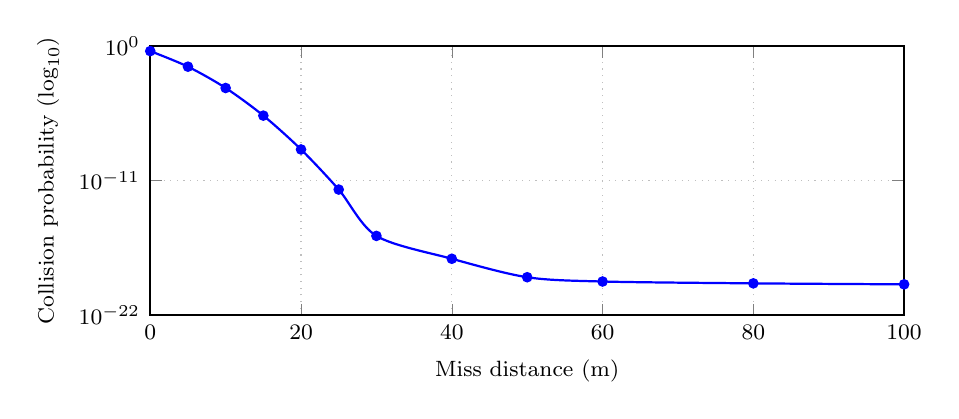
\begin{tikzpicture}
\begin{axis}[
  width=0.92\columnwidth, height=5.0cm,
  xlabel={Miss distance (m)},
  ylabel={Collision probability ($\log_{10}$)},
  xmin=0, xmax=100,
  ymode=log,
  ymin=1e-22, ymax=1,
  log basis y=10,
  xtick={0,20,40,60,80,100},
  grid=major,
  grid style={dotted,gray!50},
  thick,
  mark size=1.5pt,
  title style={font=\footnotesize},
]
\addplot[blue, mark=*, smooth] coordinates {
  (0,   3.935e-1)
  (5,   2.1e-2)
  (10,  3.8e-4)
  (15,  2.1e-6)
  (20,  3.6e-9)
  (25,  1.9e-12)
  (30,  3.1e-16)
  (40,  4.2e-18)
  (50,  1.3e-19)
  (60,  5.8e-20)
  (80,  4.1e-20)
  (100, 3.41e-20)
};
\end{axis}
\end{tikzpicture}
\caption{Corrected hard-body collision probability ($\sigma=10$~m per axis,
$\RHBR=10$~m). Probability falls sharply as miss distance increases, spanning
twenty decades from 0 to 100~m.}
\label{fig:pc_vs_miss}
\end{figure}

\subsection{Synthetic Model Performance}

\begin{table}[h]
\caption{Cached Synthetic Classification Metrics (\%)}
\label{tab:metrics}
\centering
\footnotesize
\begin{tabular}{@{}lrrrrl@{}}
\toprule
\textbf{Model} & \textbf{Acc.} & \textbf{Prec.} & \textbf{Rec.} & \textbf{F1} & \textbf{$N$} \\
\midrule
Risk Scorer (XGBoost) & 75.46 & 87.83 & 44.64 & 59.20 & 4\,096 \\
Graph Cascade (GNN)   & 98.76 & 98.46 & 98.69 & 98.57 & 2\,985 \\
GAT Cascade           & 95.54 & 94.76 & 94.98 & 94.87 & 2\,985 \\
\bottomrule
\end{tabular}
\end{table}

Fig.~\ref{fig:metrics_bar} visualizes the classification metrics. Trajectory
predictor: MAE~=~226.93~km, RMSE~=~281.74~km (768 coordinate values).

%% --- Fig 2: Classification metrics bar chart (pgfplots) ---------------------
\begin{figure}[h]
\centering
\begin{tikzpicture}
\begin{axis}[
  ybar,
  width=0.96\columnwidth, height=5.2cm,
  bar width=0.18cm,
  ylabel={Score (\%)},
  ymin=35, ymax=102,
  xtick=data,
  symbolic x coords={Accuracy,Precision,Recall,F1},
  x tick label style={font=\footnotesize, rotate=0},
  legend style={at={(0.5,1.02)}, anchor=south, legend columns=3,
                font=\scriptsize, draw=none},
  legend image code/.code={
    \draw[#1, fill=#1] (0cm,-0.1cm) rectangle (0.2cm,0.2cm);
  },
  grid=major,
  grid style={dotted,gray!40},
  enlarge x limits=0.2,
]
\addplot[fill=blue!70, draw=blue!80]
  coordinates {(Accuracy,75.46)(Precision,87.83)(Recall,44.64)(F1,59.20)};
\addplot[fill=orange!80, draw=orange!90, postaction={pattern=north east lines}]
  coordinates {(Accuracy,98.76)(Precision,98.46)(Recall,98.69)(F1,98.57)};
\addplot[fill=green!60, draw=green!70, postaction={pattern=dots}]
  coordinates {(Accuracy,95.54)(Precision,94.76)(Recall,94.98)(F1,94.87)};
\legend{Risk Scorer, Graph Cascade, GAT Cascade}
\end{axis}
\end{tikzpicture}
\caption{Classification metrics from the repository cache, regenerated through
the production scoring entry points. The two graph rankers are now distinct; the
risk scorer's low recall is disclosed rather than hidden.}
\label{fig:metrics_bar}
\end{figure}

\textit{Interpretation:} The GAT row was previously a byte-for-byte copy of the
Graph Cascade row, because \texttt{gat\_cascade.py} gated its only implementation
behind an uninstalled optional package and every prediction fell through to
\texttt{CascadeGNN}. The GAT is now a trained attention network and the two
models are genuinely distinct. The risk-scorer row is lower than earlier drafts
reported because metrics are computed through the production
\texttt{XGBoostScorer.score} entry point rather than the fallback model that never
served alerts; its 44.64\% recall means the deployed scorer misses more than half
of positives at the 0.5 threshold, which is a real limitation and not a rounding
artifact. High accuracy on the synthetic set establishes reproducibility on the
training distribution, not external validity. The attention ranker was trained on
a disjoint synthetic seed from its evaluation seed, but both derive from the same
generator, so this is a generalization check within the synthetic distribution
only. Independent time-separated splits and real CDM records are required for a
publishable operational-accuracy claim.

\subsection{Debris Envelope Radii}

\begin{table}[h]
\caption{Post-Impact Debris Envelope Radii}
\label{tab:debris_radii}
\centering
\footnotesize
\begin{tabular}{@{}cc@{}}
\toprule
\textbf{Post-impact time} & \textbf{Radius (km)} \\
\midrule
0 h (impact) & 1.500   \\
1 h          & 211.704 \\
2 h          & 319.626 \\
4 h          & 403.483 \\
8 h          & 431.414 \\
24 h         & 433.500 \\
\bottomrule
\end{tabular}
\end{table}

The asymptotic convergence reflects exponential fragment velocity decay in the
EVOLVE model; Fig.~\ref{fig:debris_envelope} shows the expansion curve.

%% --- Fig 3: Debris envelope (pgfplots) --------------------------------------
\begin{figure}[h]
\centering
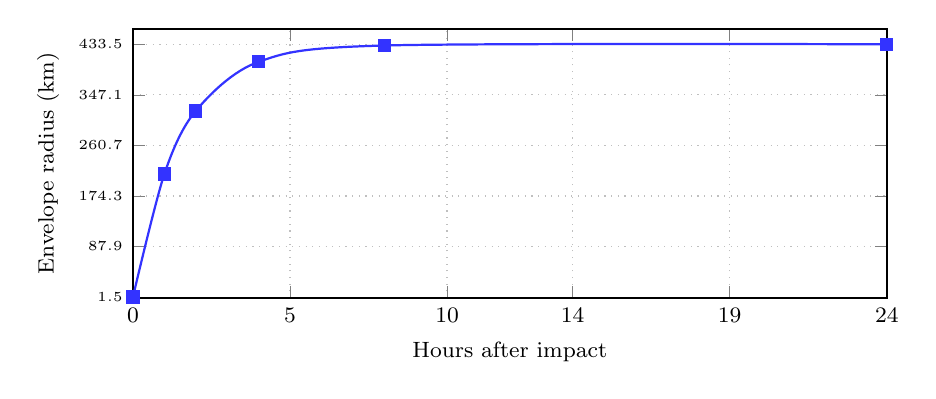
\begin{tikzpicture}
\begin{axis}[
  width=0.92\columnwidth, height=5.0cm,
  xlabel={Hours after impact},
  ylabel={Envelope radius (km)},
  xmin=0, xmax=24,
  ymin=0, ymax=460,
  xtick={0,5,10,14,19,24},
  ytick={1.5,87.9,174.3,260.7,347.1,433.5},
  yticklabel style={font=\tiny},
  grid=major,
  grid style={dotted,gray!50},
  thick,
  mark size=2pt,
]
\addplot[blue!80, mark=square*, smooth] coordinates {
  (0,  1.500)
  (1,  211.704)
  (2,  319.626)
  (4,  403.483)
  (8,  431.414)
  (24, 433.500)
};
\end{axis}
\end{tikzpicture}
\caption{Isotropic debris-envelope forecast using $r_0 = 1.5$~km,
$v_0 = 80$~m/s, $\tau = 5{,}400$~s, and a 1\,500~km cap. The asymptotic
radius below the cap reflects exponential velocity decay.}
\label{fig:debris_envelope}
\end{figure}

%% =============================================================
\section{Discussion and Limitations}
\label{sec:discussion}

\subsection{What the Prototype Demonstrates}

\begin{itemize}
  \item End-to-end path: TLE $\to$ SGP4 $\to$ Foster $\Pc$ $\to$ CPI $\to$
        XGBoost $\to$ graph cascade $\to$ Cesium globe.
  \item Transparent, auditable methodology at every stage.
  \item Deterministic injection scenarios enabling repeatable regression tests.
  \item Clear API contracts supporting modular component replacement.
\end{itemize}

\subsection{Limitations}

\begin{table}[h]
\caption{Current Limitations and Recommended Next Steps}
\label{tab:limits}
\centering
\footnotesize
\begin{tabular}{@{}p{1.5cm}p{3.0cm}p{2.7cm}@{}}
\toprule
\textbf{Domain} & \textbf{Limitation} & \textbf{Next Step} \\
\midrule
Orbit state   & TLE/SGP4 degrades with age and maneuver mismatch
              & Catalog archive with truth ephemerides \\
Uncertainty   & RTN model is analytical approximation
              & B-plane $\Pc$ validation vs.\ NASA CARA \\
Collision risk & Fixed 10~m HBR; no size catalog
              & Per-pair object dimensions \\
Debris        & Isotropic EVOLVE; no re-entry trajectory
              & Fragment orbital propagation with drag \\
ML scorer     & 44.64\% recall; same distribution in train and test
              & Independent splits; real CDM labels; retune threshold \\
Graph models  & Both rankers share one feature representation, so
              cross-checking cannot catch a common feature error
              & Independently derived feature sets \\
Scale         & Pairwise~O($N^2$); \texttt{np.add\_at} suits $10^2$ nodes
              & 27\,000-object throughput benchmarks \\
Model startup & Missing artifact triggers synchronous retraining on import
              & Pre-baked artifact; background warm-up \\
Access control & Unauthenticated commands and session minting default on;
              missing headers attributed to a shared all-agency session
              & Default both off; issue per-agency sessions \\
Persistence   & Alert and debris state is in-process; no decision audit trail
              & Durable store with decision logging \\
\bottomrule
\end{tabular}
\end{table}

\subsection{Threats to Validity}

The metric cache reflects a single deterministic generation run and may not
generalize to other seeds, class balances, or real encounter data. Two previously
identified threats are now resolved and are recorded here to prevent their
recurrence. \emph{Graph model degeneracy:} the identical GNN and GAT scores were
not a ceiling effect or limited graph diversity---the GAT's only implementation
was gated behind an uninstalled package, so one model was reported as two.
\emph{Graph ranker redundancy:} the surrogate was previously absent from the
request path; it now runs as an explicit cross-check, but the residual threat is
that a shared upstream feature error would affect both models identically and
would not be detected. \emph{Fabricated plans:} ranker failure no longer
converts to an all-zero maneuver plan. The 116 tests are narrow regression testing
of specific corrected behaviours and do not constitute comprehensive V\&{}V.
Visual correctness was assessed through code review only; no operator user study
was performed.

%% =============================================================
\section{Conclusion}
\label{sec:conclusion}

Orbital Sentinel provides a coherent, explainable prototype for real-time
orbital visualization and conjunction response. The Foster B-plane pipeline,
RTN covariance model, Hermite TCA refinement, XGBoost risk scorer, graph cascade
rankers, and NASA EVOLVE debris model are all documented to their implementation
files and grounded in established space-mechanics methods.

The audit identified eleven defects. Five concern the physics and rendering
path; six concern the learned and disseminated results: an attention ranker that
silently reported another model's scores, an alert pipeline disabled under the
default configuration, ranker failure converted into a fabricated all-zero plan,
risk-scorer metrics drawn from a model outside the request path, alert count and
list able to disagree, and TCA urgency measured against wall-clock time. All
eleven are corrected, with behavioural effects verified by a 116-test regression
suite plus an in-process check against a 120-satellite snapshot.

The methodological finding is worth separating from the individual fixes. Every
defect in the learned-component group shared one shape: the code computed
something correct and the \emph{description} of that computation was wrong. A stub
reported as a trained model, metrics attributed to a model outside the request
path, a silent fallback reported as a healthy plan, and a benchmarked model
presented as production corroboration are reporting failures rather than
computational ones. They are also the failures a synthetic test suite is least
likely to catch, because the numbers produced remain plausible. The defences
adopted in response---artifact-level independence and degeneracy flags,
disagreement thresholds surfaced to the operator, and metrics generated through
the production entry point rather than a parallel one---are therefore part of the
contribution.

Cached synthetic metrics are useful within their stated scope: 75.46\%
risk-scorer accuracy at 44.64\% recall on Foster-generated data through the
production path, 98.76\% for the surrogate ranker, and 95.54\% for the attention
ranker. The correct conclusion is that the prototype offers a reproducible
architecture, an aligned event chain from encounter detection through
visualization, and a corrected baseline for future validation---not that it
possesses operational collision-prediction accuracy. The risk scorer's recall is
a known weakness of the deployed model that must be addressed before the model
is trusted operationally. Independent temporal evaluation, real CDM data, and full
EVOLVE fragment propagation remain necessary before operational deployment.

%% =============================================================
\begin{thebibliography}{10}

\bibitem{esa2024}
European Space Agency, ``ESA's Annual Space Environment Report,''
ESA Space Debris Office, Darmstadt, Germany, 2024.

\bibitem{vallado2006}
D.~A.~Vallado, P.~Crawford, R.~Hujsak, and T.~S.~Kelso,
``Revisiting Spacetrack Report \#3,''
in \emph{Proc. AIAA/AAS Astrodynamics Specialist Conf.},
Keystone, CO, AIAA~2006-6753, 2006.

\bibitem{foster1992}
J.~L.~Foster and H.~S.~Estes,
``A Parametric Analysis of Orbital Debris Collision Probability
  and Maneuver Rate for Space Vehicles,''
NASA/JSC-25898, 1992.

\bibitem{chan1997}
F.~K.~Chan,
``Spacecraft Collision Probability,''
\emph{J.~Guidance, Control, Dyn.},
vol.~20, no.~3, pp.~566--571, 1997.

\bibitem{johnson2001}
N.~L.~Johnson, P.~H.~Krisko, J.-C.~Liou, and P.~D.~Anz-Meador,
``NASA's New Breakup Model of EVOLVE~4.0,''
\emph{Adv.~Space Res.}, vol.~28, no.~9, pp.~1377--1384, 2001.

\bibitem{alfriend1999}
K.~T.~Alfriend, M.~R.~Akella, J.~Frisbee, J.~L.~Foster,
D.~J.~Lee, and M.~Wilkins,
``Probability of Collision Error Analysis,''
\emph{Space Debris}, vol.~1, no.~1, pp.~21--35, 1999.

\bibitem{akella2000}
M.~R.~Akella and K.~T.~Alfriend,
``Probability of Collision Between Space Objects,''
\emph{J.~Guidance, Control, Dyn.}, vol.~23, no.~5, pp.~769--772, 2000.

\bibitem{battin1999}
R.~H.~Battin,
\emph{An Introduction to the Mathematics and Methods of Astrodynamics},
revised ed.
AIAA Education Series, 1999.

\bibitem{orbital_sentinel_repo}
Orbital Sentinel repository: \texttt{README.md},
\texttt{PROJECT\_SCENARIO.md}, \texttt{cascade\_planner.py},
\texttt{analytics.py}, \texttt{conjunction.py}, \texttt{debris\_model.py},
\texttt{xgboost\_scorer.py}, \texttt{gnn\_cascade.py}, \texttt{gat\_cascade.py},
source files inspected in the supplied workspace, accessed Sept.\ 2026.

\bibitem{orbital_sentinel_metrics}
Orbital Sentinel \texttt{model\_metrics\_cache.json},
synthetic evaluation artifact, generated 25~Sep.\ 2026.

\end{thebibliography}

\end{document}
